\documentclass[a4paper,oneside,openany,11pt]{memoir}
\usepackage{geometry}
\geometry{
    inner=1.5cm, % Inner margin
    outer=2cm, % Outer margin
    bindingoffset=.5cm, % Binding offset
    top=3.5cm, % Top margin
    bottom=3.5cm, % Bottom margin
    %    showframe, % Uncomment to show how the type block is set on the page
}
\linespread{1.15}

\usepackage[english]{babel}    
\usepackage{xspace}
\usepackage{microtype}    
\usepackage[utf8]{inputenc}    % Allows for writing special charachters in the tex-file 

\usepackage{amsmath,amssymb,amsfonts,dsfont,bm}     % Standard mathematics 
\allowdisplaybreaks     %Allows pagebreak during multiline math enviroments
\usepackage{mathrsfs}
\usepackage[usenames,dvipsnames]{xcolor}
\usepackage{hyperref}
\usepackage{slashed}
\usepackage{youngtab}
\usepackage{physics}
\usepackage{tensor}


\usepackage{siunitx}
\sisetup{exponent-product = \cdot, 
    separate-uncertainty} 

%Bibliography
\usepackage[sort&compress, numbers, merge]{natbib}
\setlength{\bibsep}{0.0em}
\bibliographystyle{apsrev4-1}
\addto\captionsenglish{\renewcommand*{\bibname}{\LARGE References}}
\makeatletter
%\renewcommand{\@memb@bchap}{ \section*{\bibname} \bibmark \prebibhook}
\makeatother

%Figures and tables
\usepackage{graphicx}
\graphicspath{{./Figures/}}


\counterwithout{section}{chapter} % Include if sections should be taken at the top level
\counterwithout{figure}{chapter} %Removes chapter number on figures
\setsecnumdepth{subsection}
\numberwithin{equation}{section} %Denotes that equations should be numbered a section level


\newcommand{\aaron}[1]{{\color{OliveGreen} #1}}
\newcommand{\TODO}[1]{{\color{red}[}{\color{red}TODO:} {\color{blue}#1}{\color{red}]}}
\newcommand{\NOTE}[1]{{\color{blue}[#1]}}

%Table of contents
\renewcommand{\aftertoctitle}{\par\nobreak }
\maxtocdepth{subsection}


% % % % Document % % % % 
\begin{document}

\title{\HUGE Black-hole stability in quadratic gravity: well-posed Ostrogradski notes}

\author{Hyun Lim, Aaron Held\\(work in progress)}


\maketitle

\tableofcontents*

%=======================================================================================================

\section{The Ostrogradski instability and numerical well-posedness}

Since the field equations of quadratic gravity (QG) contain higher-order (quartic) time derivatives, they exhibit an Ostrogradski instability. In this section, we will show, by use of simple examples, those field equations which exhibit an Ostrogradski instability can nevertheless have a well-posed initial value problem. Further, we will review (and give an alternative) proof that QG admits such a well-posed evolution. While this does \emph{not} show that specific solutions, e.g., the Schwarzschild metric, are stable, it guarantees that stability can be investigated numerically.

\subsection{A point-particle example}
%
\begin{figure}
  \centering
  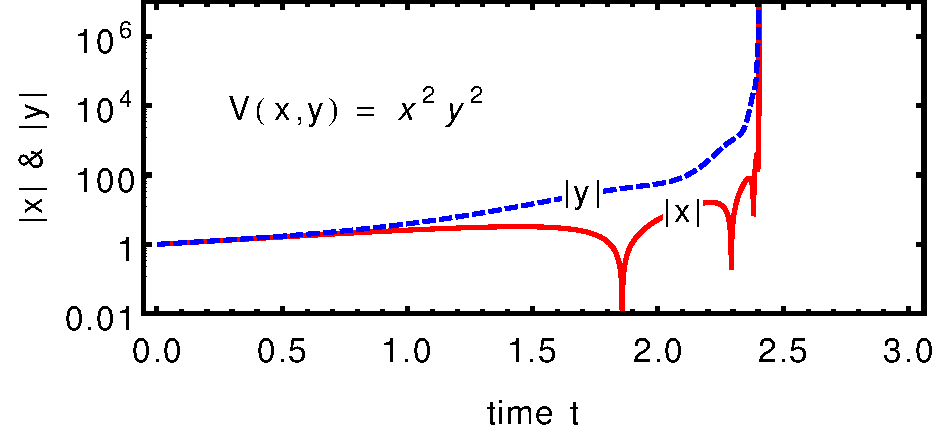
\includegraphics[width=0.49\textwidth]{pointParticle_divergenceAtFiniteTime.pdf}
  \hfill
  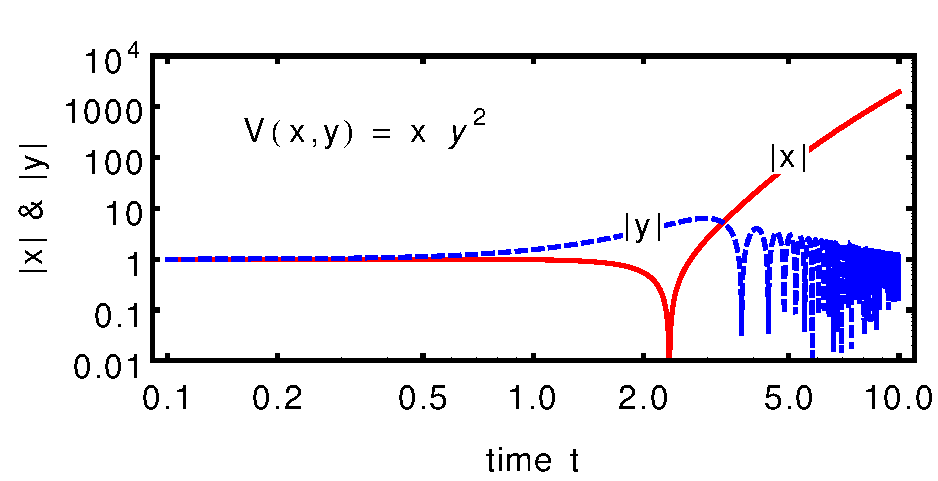
\includegraphics[width=0.49\textwidth]{pointParticle_noDivergenceAtFiniteTime.pdf}
  \caption{\label{fig:simpleExample}
  Time evolution of a point particle determined by higher-derivative equation of motion $|x(t)|$ (solid red line) and one determined by a second-order equation of motion $|y(t)|$, coupled by a potential $V(x,y) = x^2\,y^2$ and $V(x,y) = x\,y^2$ in the left-hand and right-hand panel, respectively. The left-hand case develops a divergence at finite time, but the right-hand case does not.}
\end{figure}
%
To give a first simple example, we consider a Lagrange function of two point-particles
\begin{align}
    L = \ddot{x}^2 + \dot{y}^2 + V(x,y)\;,
\end{align}
where $V(x,y)$ is a non-derivative potential. For point-particles, i.e., ordinary differential equations (ODE) determining the evolution, there is no strict notion on well-posedness \textbf{\aaron{[is that true? or do you know of one?]}}, but it can be identified with having ``no divergences at finite time'', i.e., no poles in the time evolution of $x(t)$ and $y(t)$. The higher-derivatives in $x$ result in a linear instability in the Hamiltonian \textbf{\aaron{[could explicitly add that]}}, which allows for $x$ to ``populate negative energy states''. Without interactions, i.e., for $V(x,y)=V_x(x) + V_y(y)$, this does not cause any problems and $y$ still has a ``well-posed'' evolution.
\\

However, as soon as interactions are switched on the instability transfers more and more energy from the $x$-mode into the $y$-mode since negative energies are favored in $x$ and positive ones in $y$. While overall energy is conserved, arbitrary amounts of energy can be shifted into the $y$-mode -- the onset of the Ostrogradski instability. Typically, this results in a divergence at finite time and prohibits ``well-posed'' numerical evolution. One such example is $V(x,y) = x^2\,y^2$, cf.~left-hand panel in Fig.~\ref{fig:simpleExample}.
\\
Although the instability always exists, specific choices of potential can lead to an evolution which only develops a divergence at infinite time. One such example is $V(x,y) = x\,y^2$, cf.~right-hand panel in Fig.~\ref{fig:simpleExample}. In such cases, the evolution is both Ostrogradski-instable and nevertheless well-posed. The energy that the Ostrdgradski $x$-mode feeds into the regular $y$-mode is stored in oscillations.

\subsection{Coupled scalar-field theory model}

%
\begin{figure}
  \centering
  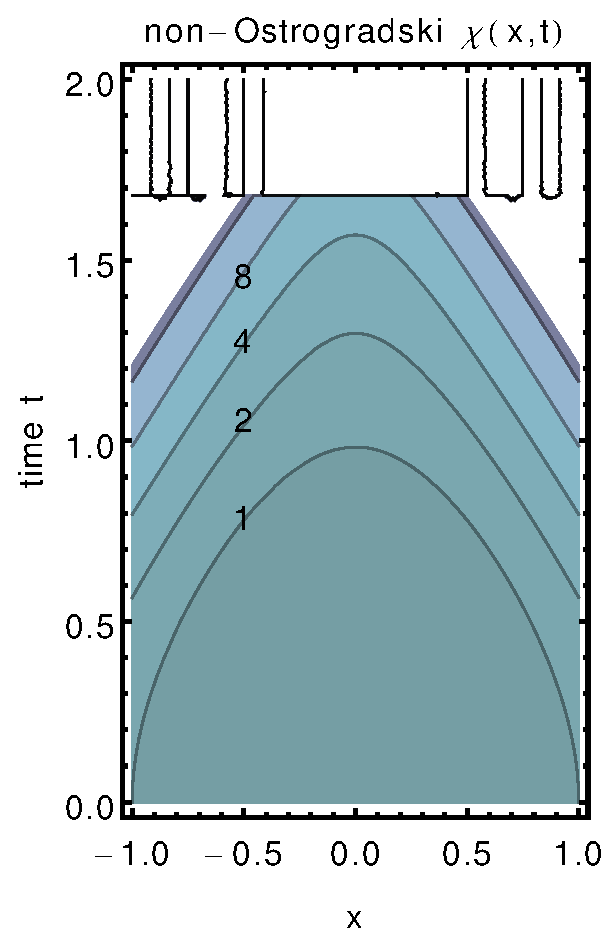
\includegraphics[width=0.255\textwidth]{scalarField_divergenceAtFiniteTime_nonOstrogradskiMode.pdf}
  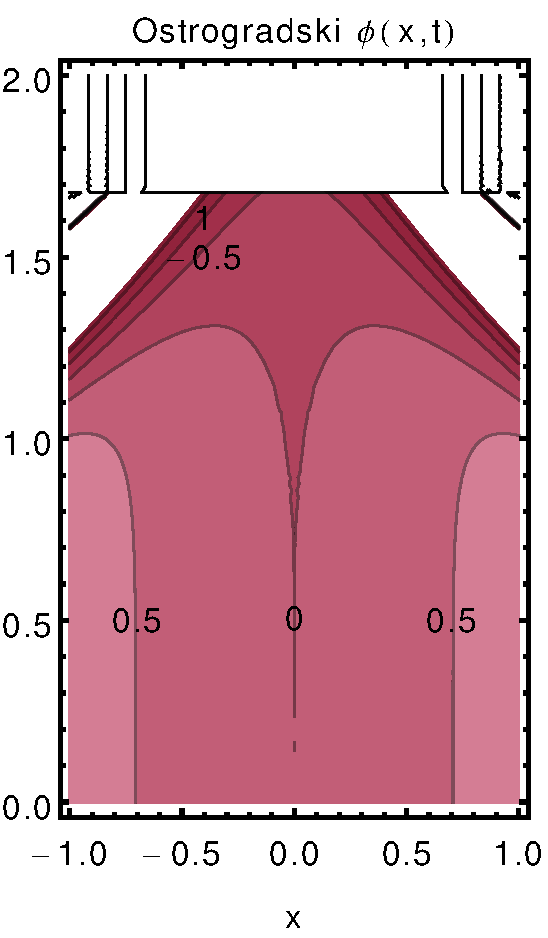
\includegraphics[width=0.23\textwidth]{scalarField_divergenceAtFiniteTime_ostrogradskiMode.pdf}
  \hfill\vline\hfill
  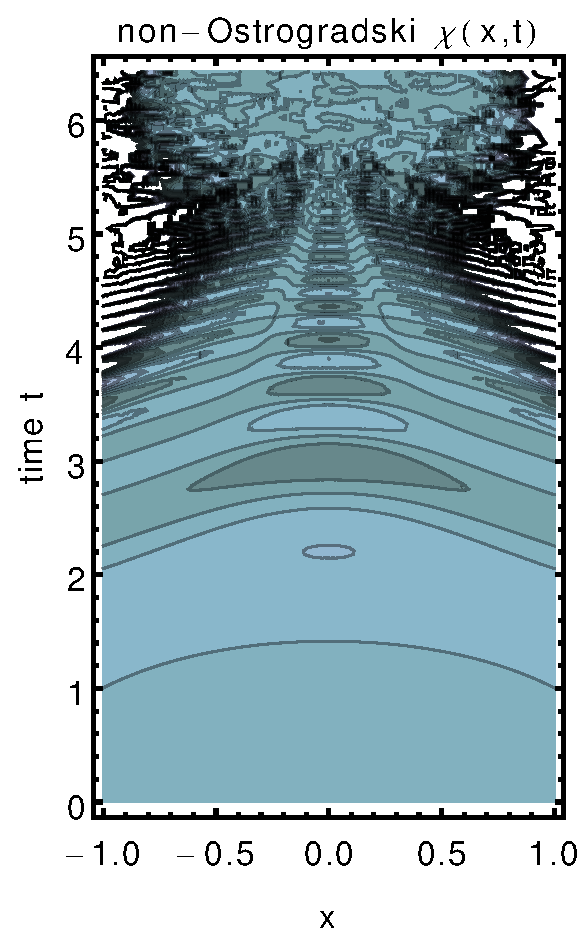
\includegraphics[width=0.245\textwidth]{scalarField_noDivergenceAtFiniteTime_nonOstrogradskiMode.pdf}
  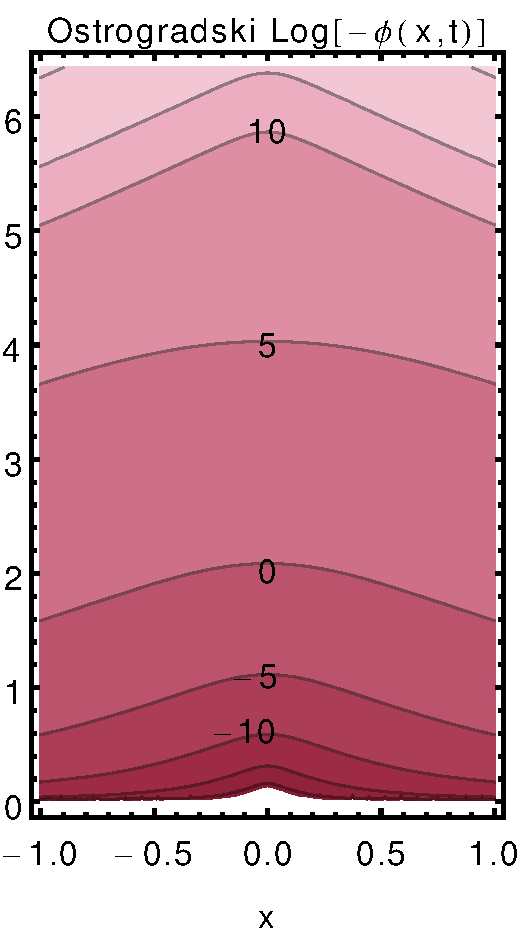
\includegraphics[width=0.22\textwidth]{scalarField_noDivergenceAtFiniteTime_ostrogradskiMode.pdf}
  \caption{\label{fig:scalarFieldExample}
  Time evolution of two coupled scalar fields determined by higher-derivative equation of motion for $\phi$ and one second-order equation of motion for $\chi$, coupled by a potential $V(\phi,\chi) = \phi^2\,\chi^2$ (two left-hand panels) and $V(\phi,\chi) = \phi\,\chi^2$ (two right-hand panels). The left-hand case develops a divergence at finite time, but the right-hand case does not.}
\end{figure}
%


This simple example can be extended to the time evolution of a 1+1 dimensional coupled scalar-field theory governed by a partial differential equation (PDE). Its Lagrangian reads
\begin{align}
    \mathcal{L} = \frac{1}{2}\left(\Box \phi\right)\left(\Box \phi\right) - \frac{1}{2}\chi\left(\Box \chi\right) + V(\phi,\,\chi)\;,
\end{align}
where $\phi(x,t)$ and $\chi(x,t)$ are two real scalar fields, $\Box = \partial_t^2 - \partial_x^2$, and $V(\phi,\,\chi)$ is an a priori arbitrary non-derivative potential. The equations of motion read
\begin{align}
\label{eq:eoms_scalarFieldExample}
    \Box\left(\Box \phi\right) &= -\partial_\phi\,V(\phi,\,\chi)\;,\\
    \Box \chi &= -\partial_\chi\,V(\phi,\,\chi)\;.
\end{align}
Here, $\phi$ corresponds to a higher-derivative scalar and $\chi$ is a usual scalar field. Again, if the potential decouples, i.e., $V(\phi,\,\chi) = V_\phi(\phi) + V_\chi(\chi)$, the time evolution is obviously well defined everywhere.
Fig.~\ref{fig:scalarFieldExample} again depicts two cases of time evolution: $V(\phi,\,\chi) = \phi^2\,\chi^2$ for which the Ostrigradski instability results in a divergence at finite time, beyond which the PDE evolution breaks down (not well-posed), but also one , i.e., $V(\phi,\,\chi) = \phi\,\chi^2$, for which the PDE evolution despite an the onset of an Ostrogradski instability does not develop a divergence at finite time (well-posed). As initial conditions we choose $\phi(x,t=0)= x^2$ and $\phi(x,t=0)= 0$ in the left-hand and right-hand panel, respectively. The other initial conditions are chosen as $\phi(x,t=0)= x^2$, $\dot{\phi}(x,t=0) = \ddot{\phi}(x,t=0) = \dddot{\phi}(x,t=0) = 0$, $\chi(x,t=0)= x^2$, and $\dot{\chi}(x,t=0)=0$ in both cases. Again, the energy that the Ostrdgradski $\phi$-mode feeds into the regular $\chi$-mode is stored in oscillations.
\\

The equations of motion can be cast into an extended sytstem with only first-order time derivatives by defining $\zeta \equiv \Box \phi$ and thereupon $\nu_\phi = \partial_t\phi$, $\nu_\chi = \partial_t\chi$, and $\nu_\zeta = \partial_t\zeta$. Moreover, defining the vectors $v = (\phi,\,\chi,\,\zeta)^T$ and $w = (\nu_\phi,\,\nu_\chi,\,\nu_\zeta)^T$, we can rewrite Eq.~\eqref{eq:eoms_scalarFieldExample} as
\begin{align}
    \partial_t\,v &= A\,w\;,
    \qquad\qquad\qquad
    \partial_t\,w = B\,\partial_x^2\,v + \mathcal{V}(\phi,\,\chi,\,\zeta)\;.
    \\\notag
    \text{where:}\; A&=B=\begin{pmatrix}1&0&0\\0&1&0\\0&0&1\end{pmatrix}\,\qquad
     \mathcal{V}=\begin{pmatrix}\zeta\\ \partial_\phi\,V(\phi,\chi)\\ \partial_\chi\,V(\phi,\chi)\end{pmatrix}\;.
\end{align}
\textbf{\aaron{[If $\mathcal{V}$ were not non-linear, this system would be of ``Gundlach--Maritn-Garcia form'' \cite{Gundlach:2005ta}. Then, I would know how to put explicit conditions for well-posedness. Do you know how to do that for quartic potentials?]}}


\bibliography{References}
    
\end{document}



